\chapter{集合函数与子集累计}
\label{chap:set-functions}
\label{chap:graph-set-functions}

在一片区域里安装传感器时，每个候选位置覆盖一块范围，相邻位置的覆盖范围往往重叠。选定一组位置后，有意义的是这组位置合起来覆盖了多少，而不是各自覆盖面积的简单相加。从一批特征里挑出一组、从一张图里挑出一部分顶点，评价的也都是整组选择。本章要回答两个问题：怎样描述这种对整组的评价，以及评价具有哪些结构可以供后面的选择算法利用；另外，已知每个子集的累计评价时，怎样恢复各个子集自身的贡献。

前两节建立描述子集评价的语言。第~\ref{sec:graph-set-function-basics}节把“给子集赋值”写成集合函数，用指示向量换一种方式索引子集，并用加入一个元素前后的评价差定义边际增益。第~\ref{sec:graph-set-function-properties}节用边际增益区分单调性、模性和次模性，并说明它们互不蕴含。

第~\ref{sec:comb-cumulative-inversion}节处理另一项任务：由累计值恢复自身贡献。它只用有限求和与包含关系，不依赖前一节的任何性质，也不是后两章选择算法的前提。本章用到卷一的幂集计数、裂项求和、偏序关系、有限和的交换次序与组合数的交错和，用到时在当地说明所需的结论。

% 第8章第1节：集合函数（集合函数的定义；子集与二值向量；边际增益）。

\section{集合函数}
\label{sec:graph-set-function-basics}

给每个元素赋一个数，只需要一张长度为元素个数的表。对整组选择打分就不同了：元素之间的重叠、替代或配合都会改变总分，分数只能直接对子集给出。所以本节以子集为自变量的函数为基本对象。选择又往往是一次加入一个元素，所以还要看加入一个元素前后分数怎样变化。

\subsection{集合函数的定义}
\label{sec:graph-setfn-definition}

图~\ref{fig:graph-setfn-sensor-coverage}是一块由上下两行、左右八列组成的区域，共$16$个格子。有四个候选传感器：$a$覆盖第$2$至$6$列的$10$个格子，$b$覆盖第$1$至$4$列的$8$个格子，$c$覆盖第$5$至$8$列的$8$个格子，$d$只覆盖左上角的$1$个格子。

选定一组传感器后，我们关心它们合起来覆盖了多少个不同的格子。记传感器$v$覆盖的格子集合为$C_v$，选定的传感器集合为$S$，覆盖量就是
\[
  F(S)=\Bigl|\bigcup_{v\in S}C_v\Bigr|.
\]
单独看，$F(\{a\})=10$，$F(\{b\})=8$。两者一起时，第$2$至$4$列被重复覆盖，所以
\[
  F(\{a,b\})=12<F(\{a\})+F(\{b\})=18.
\]
整组的价值不能由各成员的价值相加得到，因此评价必须直接以“哪些传感器被选中”为输入。本章和下一章都用这个实例做算例。

\begin{figure}[!htb]
  \centering
  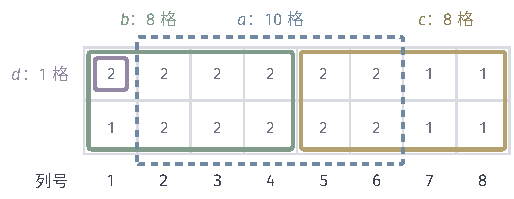
\includegraphics[width=87.027mm]{figures/01-basic-mathematics/04-graphs/tikz/c4-sensor-coverage/figure.pdf}
  \caption{贯穿本章和下一章的传感器覆盖实例。区域由$2\times 8$个格子组成；绿色框为$b$（第$1$至$4$列），黄色框为$c$（第$5$至$8$列），蓝色虚线框为$a$（第$2$至$6$列），紫色小框为$d$（左上角一格）。格内数字是覆盖该格的传感器个数，数字$2$所在的格子都被重复覆盖，因而各传感器覆盖格数之和大于它们合起来覆盖的格数。}
  \label{fig:graph-setfn-sensor-coverage}
\end{figure}

覆盖量的输入是一个子集，输出是一个实数。把这种对应一般化，就得到下面的定义。

\begin{definition}[集合函数]
\label{def:graph-setfn-set-function}
设$V$是有限集合，称为\term{底集}（ground set）。把$V$的每个子集对应到一个实数的映射
\[
  F:\mathcal P(V)\to\mathbb R
\]
称为$V$上的\term{集合函数}（set function），其中$\mathcal P(V)$是$V$的幂集。
\end{definition}

定义要求$F$在每个子集上都有值，包括空集。空集表示“什么都不选”，它的值是比较其他选择的起点：覆盖量取$F(\varnothing)=0$，一个带固定开销的评价则可能取非零值。底集中的元素可以是传感器、特征、顶点或边；集合函数本身并不要求底集带有图结构。

\paragraph{总成本与割权}
同一个子集可以按不同目的评价。给四个传感器依次指定安装成本$4,3,4,1$（对应$a,b,c,d$），总成本
\[
  c(S)=\sum_{v\in S}c_v
\]
是一个集合函数，例如$c(\{a,b\})=7$；覆盖量$F$是另一个，$F(\{a,b\})=12$。

第三个例子来自图。设$\mathcal G=(V,E)$是无向图，每条边$\{i,j\}$带非负权$w_{i,j}$。顶点子集$S$把顶点分成$S$与$V\setminus S$两侧，这就是第~\ref{sec:graph-opt-cut-property}节所说的割；那里要求两侧都非空，这里允许$S=\varnothing$或$S=V$，这时没有边跨越两侧。两端分居两侧的边的权之和
\[
  \operatorname{cut}(S)=\sum_{\{i,j\}\in E:\ |\{i,j\}\cap S|=1}w_{i,j}
\]
称为$S$的割权，它以顶点子集为自变量。

三个函数分别累计单项成本、合并覆盖范围、统计跨越两侧的边，元素之间的相互影响各不相同。下一节据此区分它们的性质。

\paragraph{取值表与求值规则}
$n$元底集的每个元素有选与不选两种可能，按乘法规则共有$2^n$个子集，所以一个集合函数的完整取值表有$2^n$项（幂集计数可参考\BookChapterRef{chap:counting}{卷一“计数”章}）。传感器实例只有$16$项。除上面的单元素值外，二元子集的覆盖量为
\[
  \begin{gathered}
  F(\{a,b\})=12,\quad F(\{a,c\})=14,\quad F(\{a,d\})=11,\\
  F(\{b,c\})=16,\quad F(\{b,d\})=8,\quad F(\{c,d\})=9,
  \end{gathered}
\]
三元子集中$\{a,b,c\}$与$\{b,c,d\}$覆盖全部$16$格；后面各节的枚举基准都从这些值读出。

底集有$50$个元素时，取值表已超过$10^{15}$项，无法存储。因此实际问题中的集合函数通常由一条规则给出：给定$S$，按规则算出$F(S)$，这样的一次计算称为一次\emph{求值}。覆盖量的规则是维护一个格子标记数组，初始全为未覆盖，依次标记$S$中各传感器覆盖的格子，最后计数。求$F(\{a,b,c\})$时，读入$b$标记第$1$至$4$列，读入$a$新增第$5$、$6$列，读入$c$新增第$7$、$8$列，共$16$格，工作量与$\sum_{v\in S}|C_v|$成正比。割权的规则是扫描全部边，工作量与边数成正比。

两种给出方式的代价不同。查表读值便宜，但表随$n$指数增长；规则不必存表，却每次读值都要计算。所以后面分析算法时，我们把求值次数和每次求值的代价分开计算，不把求值视为免费。

\subsection{子集与二值向量}
\label{sec:graph-setfn-binary-vectors}

给底集的元素固定编号$V=\{1,\ldots,n\}$。前面计算子集个数时用到，子集$S$与长度为$n$的零一记录一一对应。把这条记录写成向量$\bm x=(x_1,\ldots,x_n)\in\{0,1\}^n$，其中
\[
  x_i=\mathbb I\{i\in S\},
\]
称$\bm x$为$S$的\term{指示向量}（indicator vector）。这里$\mathbb I\{\cdot\}$是指示函数，条件成立时取$1$，否则取$0$。反过来，收集取值为$1$的坐标就恢复出子集：$S=\{i:x_i=1\}$。

集合运算在指示向量上逐坐标进行。设$S,T$的指示向量为$\bm x,\bm y$，则$|S|=\sum_ix_i$；并集、交集与补集的第$i$个坐标依次是
\[
  \max\{x_i,y_i\},\qquad \min\{x_i,y_i\}=x_iy_i,\qquad 1-x_i;
\]
包含关系$S\subseteq T$对应逐坐标的$x_i\leq y_i$。每种运算都只需扫描一遍$n$个坐标。

于是集合函数也可以写成二值向量的函数：令$f(\bm x)=F(\{i:x_i=1\})$，$f$与$F$只是同一组数值的两种索引方式。图~\ref{fig:graph-setfn-subset-binary-cube}以三元底集为例画出这一对应：八个子集恰好是立方体的八个顶点，立方体的每条边连接只差一个元素的两个子集，也就是只差一个坐标的两个向量。

\begin{figure}[!htb]
  \centering
  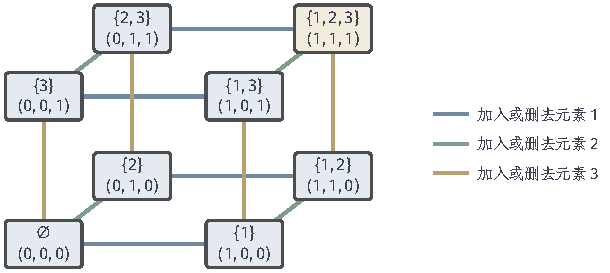
\includegraphics[width=103.209mm]{figures/01-basic-mathematics/04-graphs/tikz/c4-subset-binary-cube/figure.pdf}
  \caption{三元底集$V=\{1,2,3\}$的八个子集与指示向量$(x_1,x_2,x_3)$排成立方体的顶点。每个框上行是子集，下行是对应的向量；边的颜色表示沿这条边加入或删去哪个元素，也就是改变哪个坐标。沿任一条边向上走一步，就是在当前子集中加入一个元素。}
  \label{fig:graph-setfn-subset-binary-cube}
\end{figure}

这一改写只换了表示方式，并没有带来额外结构。写成$f(\bm x)$之后，$f$不一定是各坐标的函数之和，也不一定能分解成只读取少数坐标的局部项；在$\{0,1\}^n$上谈连续性或求导也没有意义。第~\ref{chap:pairwise-binary-minimization}章和第~\ref{part:graph-dynamic-programming}部分讨论的，正是函数确实具有某种局部分解时可以怎样利用它。

\subsection{边际增益}
\label{sec:graph-setfn-marginal-gain}

选择子集时，最直接的问题是：在已经选好的集合上再加一个元素，评价会改变多少。

\begin{definition}[边际增益]
\label{def:graph-setfn-marginal-gain}
设$F$是$V$上的集合函数，$S\subseteq V$，$v\in V\setminus S$。称
\begin{equation}
  \Delta(v\mid S)=F(S\cup\{v\})-F(S)
  \label{eq:graph-setfn-marginal-gain}
\end{equation}
为元素$v$相对于集合$S$的\term{边际增益}（marginal gain）。
\end{definition}

边际增益同时依赖新元素和已选集合。图~\ref{fig:graph-setfn-marginal-gain-overlap}比较同一个传感器$c$在两种情况下的增益。从空集加入时，$c$的$8$个格子都是新覆盖的；已经选了$a$之后，$c$的第$5$、$6$列已被$a$覆盖，只有第$7$、$8$列的$4$个格子是新的。两个增益分别是
\[
  \Delta(c\mid\varnothing)=8,\qquad \Delta(c\mid\{a\})=4.
\]
所以谈论一个元素“值多少”时，必须说明是相对于哪个已选集合。

\begin{figure}[!htb]
  \centering
  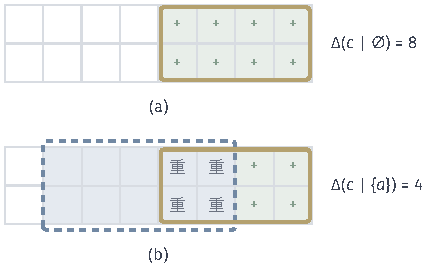
\includegraphics[width=81.217mm]{figures/01-basic-mathematics/04-graphs/tikz/c4-marginal-gain-overlap/figure.pdf}
  \caption{同一传感器$c$（黄色框）的边际增益随已选集合变化。(a) 已选集合为空，$c$覆盖的$8$个格子（绿色，标“$+$”）全部是新覆盖；(b) 已选$\{a\}$（蓝色底与蓝色虚线框），$c$与$a$重叠的第$5$、$6$列（标“重”）不再计数，只有第$7$、$8$列的$4$个格子是新覆盖。}
  \label{fig:graph-setfn-marginal-gain-overlap}
\end{figure}

\paragraph{逐个加入的累计}
边际增益只描述一步。两个有包含关系的集合相差若干元素时，把多出的元素逐个加入，函数的总变化就是一串边际增益之和。设$A\subseteq B\subseteq V$，把$B\setminus A$中的元素按任意次序排成$v_1,\ldots,v_r$，记$A_0=A$，$A_k=A\cup\{v_1,\ldots,v_k\}$。于是$A_r=B$，并且
\begin{equation}
  \begin{aligned}
  F(B)-F(A)&=\sum_{k=1}^{r}\bigl(F(A_k)-F(A_{k-1})\bigr)\\
  &=\sum_{k=1}^{r}\Delta(v_k\mid A_{k-1}).
  \end{aligned}
  \label{eq:graph-setfn-telescoping}
\end{equation}
第一个等号是裂项求和：中间的$F(A_1),\ldots,F(A_{r-1})$各出现一次正号、一次负号而抵消，只剩$F(A_r)-F(A_0)$（有限和的裂项可参考\BookChapterRef{chap:sets-relations-maps}{卷一“集合、关系与映射”章}）。第二个等号成立，是因为$A_k=A_{k-1}\cup\{v_k\}$且$v_k\notin A_{k-1}$，每一项正是一个有定义的边际增益。下一节判别性质、第~\ref{sec:graph-cardinality-selection}节分析贪心算法，用的都是这个式子。

在传感器实例中取$A=\varnothing$、$B=\{a,b,c\}$。按$a,c,b$的次序加入：$a$覆盖$10$格，$c$补上第$7$、$8$列的$4$格，$b$只补上第$1$列的$2$格，增益依次是$10,4,2$。按$b,c,a$的次序加入：$b$覆盖$8$格，$c$与$b$不重叠，补上$8$格，此时$16$格已全部覆盖，$a$的增益为$0$，增益依次是$8,8,0$。两种次序的增益之和都等于同一个值：
\[
  10+4+2=8+8+0=16=F(\{a,b,c\}).
\]
总变化由两端的集合决定，单步增益则取决于走哪条路线。

单步增益的大小也不能说明一个元素是否值得选。在空集上，$a$的增益$10$是四个传感器中最大的，但只能选两个传感器时，最好的组合是覆盖全部$16$格的$\{b,c\}$，并不包含$a$。第~\ref{sec:graph-cardinality-selection}节会具体比较这两者。

% 第8章第2节：集合函数的性质（单调性；模性；次模性；性质之间的关系）。

\section{集合函数的性质}
\label{sec:graph-set-function-properties}

上一节的三个函数在加入一个元素时表现不同：加入传感器不会减少覆盖，但新增的覆盖可能越来越少；加入一项成本总是增加固定的数额；把一个顶点移到$S$一侧，割权可能增加也可能减少。这三种表现分别对应单调性、模性和次模性。

三者都可以用边际增益判别，但各自回答一个不同的问题：新增元素会不会降低评价，每个元素的贡献是否固定，收益是否随已选集合增大而递减。所以一个函数可以具备其中任意几项而缺少其他几项，本节最后用反例和对照表核对这一点。

\subsection{单调性}
\label{sec:graph-setfn-monotonicity}

多装一个传感器，覆盖的格子只会增加或保持不变。把这一性质写成子集之间的比较，就是下面的定义。

\begin{definition}[单调非减]
\label{def:graph-setfn-monotone}
若对任意$A\subseteq B\subseteq V$都有$F(A)\leq F(B)$，称集合函数$F$\term{单调非减}（monotone nondecreasing），简称单调。
\end{definition}

定义比较的是任意两个有包含关系的子集，直接检查要考虑很多对。借助式~\eqref{eq:graph-setfn-telescoping}，可以化成只检查单个元素的条件：$F$单调，当且仅当对每个$S\subseteq V$和每个$v\notin S$都有
\[
  \Delta(v\mid S)\geq0.
\]

必要性只需取$A=S$、$B=S\cup\{v\}$。充分性：对任意$A\subseteq B$，式~\eqref{eq:graph-setfn-telescoping}把$F(B)-F(A)$写成若干个边际增益之和，每一项都非负，所以$F(A)\leq F(B)$。

覆盖量是单调的，因为加入$v$后新增的格子数
\[
  \Delta(v\mid S)=\Bigl|C_v\setminus\bigcup_{u\in S}C_u\Bigr|
\]
不会是负数。

但目标中含有覆盖量，并不保证整个目标单调。把覆盖量减去安装成本，得到净收益$G(S)=F(S)-c(S)$。比较两个集合：
\[
  G(\{b\})=8-3=5,\qquad G(\{b,d\})=8-4=4.
\]
$d$覆盖的那一格已被$b$覆盖，加入$d$不增加覆盖，却多花$1$个单位成本，所以净收益下降。

\paragraph{非负性与归一化}
函数值全为非负，也不能推出单调。在二元底集$\{1,2\}$上取
\[
  F(\varnothing)=1,\quad F(\{1\})=3,\quad F(\{2\})=2,\quad F(\{1,2\})=2,
\]
四个值都是正数，但$\Delta(2\mid\{1\})=2-3=-1<0$，所以它不单调。

反过来，单调也不能推出$F(\varnothing)=0$：常数函数$F\equiv5$是单调的。$F(\varnothing)=0$称为\emph{归一化}，它是一项约定，不是函数的固有性质：对任意集合函数，减去常数$F(\varnothing)$就得到归一化的函数，而所有边际增益保持不变。归一化且单调的函数必然处处非负，因为$F(S)\geq F(\varnothing)=0$。

\subsection{模性}
\label{sec:graph-setfn-modularity}

总成本$c(S)$具有最简单的结构：每个元素贡献一个固定的数，彼此互不影响。一般地，取常数$c_0$和每个元素的权$w_v$，令
\begin{equation}
  F(S)=c_0+\sum_{v\in S}w_v .
  \label{eq:graph-setfn-modular-form}
\end{equation}
这时对任意$S$和$v\notin S$都有
\[
  \Delta(v\mid S)=w_v,
\]
增益与已选集合无关。由上一小节的判别条件，这样的$F$单调当且仅当每个$w_v\geq0$；常数$c_0$不影响任何边际增益。

给定一个集合函数，要判断它是否具有这种固定贡献的形式，可以逐个检查边际增益是否与$S$无关；更紧凑的办法是检查一个只涉及四个函数值的等式。

对形如式~\eqref{eq:graph-setfn-modular-form}的函数和任意两个子集$A,B$，比较$F(A)+F(B)$与$F(A\cup B)+F(A\cap B)$。两边都含两个常数$c_0$，只需逐个元素比较权重被计了几次。对一个元素$v$：若$v$同时属于$A$和$B$，则$w_v$在左边计两次，在右边的并集与交集中也各计一次；若$v$只属于其中一个，则$w_v$在两边都只计一次；若$v$都不属于，则两边都不计。所以
\begin{equation}
  F(A)+F(B)=F(A\cup B)+F(A\cap B).
  \label{eq:graph-setfn-modular-equality}
\end{equation}
对所有$A,B\subseteq V$满足式~\eqref{eq:graph-setfn-modular-equality}的集合函数称为\term{模函数}（modular function）。

反过来，模等式也足以恢复固定权重的表示，所以可以用它判断元素之间有没有交互。设$F$是模函数，取$S\neq\varnothing$与$v\in S$，在式~\eqref{eq:graph-setfn-modular-equality}中令$A=S\setminus\{v\}$、$B=\{v\}$，这时$A\cup B=S$，$A\cap B=\varnothing$，得到
\[
  F(S)=F(S\setminus\{v\})+\bigl(F(\{v\})-F(\varnothing)\bigr).
\]
对$|S|$归纳，就得到
\[
  F(S)=F(\varnothing)+\sum_{v\in S}\bigl(F(\{v\})-F(\varnothing)\bigr),
\]
即式~\eqref{eq:graph-setfn-modular-form}取$c_0=F(\varnothing)$、$w_v=F(\{v\})-F(\varnothing)$。所以模函数恰好就是固定贡献形式的函数，权重可以直接从空集和单元素集的值读出。

覆盖量不是模函数。取$A=\{a\}$、$B=\{b\}$，模等式两边分别是
\[
  F(\{a\})+F(\{b\})=18,\qquad F(\{a,b\})+F(\varnothing)=12,
\]
等式不成立；差值$6$正是第$2$至$4$列被重复计数的格子。总成本则满足模等式，例如$c(\{a\})+c(\{b\})=7=c(\{a,b\})+c(\varnothing)$。

\subsection{次模性}
\label{sec:graph-setfn-submodularity}

次模性说的是收益递减：已经拥有的越多，再添一样东西带来的好处越少。覆盖量正是这样：已覆盖的格子越多，新传感器能补上的格子越少。在图~\ref{fig:graph-setfn-marginal-gain-overlap}的基础上再加入$b$，$c$的增益依次为
\[
  \Delta(c\mid\varnothing)=8,\qquad \Delta(c\mid\{a\})=4,\qquad \Delta(c\mid\{a,b\})=4,
\]
最后一步没有继续变小，但也没有变大。把“不会变大”作为要求，就得到边际收益递减的条件。

\begin{definition}[次模函数]
\label{def:graph-setfn-submodular}
若对任意$A\subseteq B\subseteq V$和任意$v\in V\setminus B$都有
\begin{equation}
  \Delta(v\mid A)\geq\Delta(v\mid B),
  \label{eq:graph-setfn-diminishing-returns}
\end{equation}
称集合函数$F$是\term{次模}函数（submodular function）。
\end{definition}

条件中的$v$不属于$B$，从而也不属于$A$，两个增益都有定义。

式~\eqref{eq:graph-setfn-diminishing-returns}要对每一对嵌套集合和每个外部元素检查。次模性还有一种不出现边际增益的写法，它和模等式形式相同，只是把等号换成不等号。

\begin{theorem}[次模性的两种刻画]
\label{thm:graph-setfn-submodular-equivalence}
设$V$是有限集合，$F$是$V$上的集合函数。$F$满足式~\eqref{eq:graph-setfn-diminishing-returns}，当且仅当对任意$X,Y\subseteq V$都有
\begin{equation}
  F(X)+F(Y)\geq F(X\cup Y)+F(X\cap Y).
  \label{eq:graph-setfn-submodular-inequality}
\end{equation}
\end{theorem}

\begin{proof}
先设式~\eqref{eq:graph-setfn-submodular-inequality}成立。给定$A\subseteq B$和$v\notin B$，取$X=A\cup\{v\}$、$Y=B$。由$A\subseteq B$得$X\cup Y=B\cup\{v\}$；由$v\notin B$得$X\cap Y=A$。代入式~\eqref{eq:graph-setfn-submodular-inequality}，
\[
  F(A\cup\{v\})+F(B)\geq F(B\cup\{v\})+F(A),
\]
移项即$\Delta(v\mid A)\geq\Delta(v\mid B)$。

再设式~\eqref{eq:graph-setfn-diminishing-returns}成立。给定$X,Y$，记$C=X\cap Y$，把$Y\setminus X$中的元素按任意次序排成$y_1,\ldots,y_r$。分别从$X$和从$C$出发逐个加入这些元素，由式~\eqref{eq:graph-setfn-telescoping}，
\[
  \begin{gathered}
  F(X\cup Y)-F(X)=\sum_{k=1}^{r}\Delta\bigl(y_k\mid X\cup\{y_1,\ldots,y_{k-1}\}\bigr),\\
  F(Y)-F(C)=\sum_{k=1}^{r}\Delta\bigl(y_k\mid C\cup\{y_1,\ldots,y_{k-1}\}\bigr).
  \end{gathered}
\]
这里用到$X\cup(Y\setminus X)=X\cup Y$与$C\cup(Y\setminus X)=Y$。对每个$k$，$C\cup\{y_1,\ldots,y_{k-1}\}\subseteq X\cup\{y_1,\ldots,y_{k-1}\}$，且$y_k$不属于后者（$y_k\notin X$，并且与前面的$y_j$不同）。由式~\eqref{eq:graph-setfn-diminishing-returns}，第二个和的每一项不小于第一个和的对应项，所以
\[
  F(X\cup Y)-F(X)\leq F(Y)-F(C),
\]
移项即得式~\eqref{eq:graph-setfn-submodular-inequality}。
\end{proof}

两种刻画用途不同：式~\eqref{eq:graph-setfn-diminishing-returns}直接对应“收益递减”的直观，适合分析逐个加入元素的算法；式~\eqref{eq:graph-setfn-submodular-inequality}只涉及四个函数值，适合验证具体函数。

两种刻画也给出构造次模函数的办法。模函数在式~\eqref{eq:graph-setfn-submodular-inequality}中处处取等号，所以是次模的。若干个函数各自满足式~\eqref{eq:graph-setfn-diminishing-returns}时，把这些不等式逐项相加，可知它们的和也满足；所以次模函数之和仍是次模函数，次模函数加上模函数也仍是次模函数。

\paragraph{覆盖函数}
覆盖量是次模的。设$A\subseteq B$，$v\notin B$。$v$相对于$S$的增益是$C_v$中尚未被$S$覆盖的格子数，即
\[
  \Delta(v\mid S)=|C_v\setminus U(S)|,\qquad U(S)=\bigcup_{u\in S}C_u.
\]
由$A\subseteq B$得$U(A)\subseteq U(B)$，于是
\[
  C_v\setminus U(B)\subseteq C_v\setminus U(A),
\]
取元素个数就得到式~\eqref{eq:graph-setfn-diminishing-returns}。

这个论证不依赖格子的具体排列，只用到“增益是$C_v$中尚未被覆盖的部分”。所以任何“覆盖了多少个不同对象”的函数都是次模的，这样的函数称为\term{覆盖函数}（coverage function）。

覆盖函数还让四值不等式有一个逐格的读法。$F(X)+F(Y)$对每个格子数两次：$X$覆盖它就计$1$，$Y$覆盖它再计$1$；$F(X\cup Y)+F(X\cap Y)$则按$X\cup Y$与$X\cap Y$是否覆盖它来数。

固定一个格子，记$p,q,r\in\{0,1\}$分别表示$X$、$Y$、$X\cap Y$是否覆盖它。$X\cup Y$覆盖它当且仅当$p,q$中至少一个为$1$，所以左边计$p+q$，右边计$\max\{p,q\}+r$，两者之差是
\[
  (p+q)-\bigl(\max\{p,q\}+r\bigr)=\min\{p,q\}-r.
\]
$X\cap Y$中的传感器同时属于$X$和$Y$，它覆盖的格子$X$与$Y$都覆盖，所以$r\leq\min\{p,q\}$，每个格子的差都不小于$0$。

差为$1$的格子恰好是$X$与$Y$都覆盖、而公共部分$X\cap Y$不覆盖的格子：两组各用自己的传感器覆盖了同一格。

图~\ref{fig:graph-setfn-submodular-overlap-count}取$X=\{a,b\}$、$Y=\{b,c\}$。第$1$至$4$列由公共的$b$覆盖，两边都计$2$；第$7$、$8$列只有$Y$覆盖，两边都计$1$；第$5$、$6$列由$X$中的$a$和$Y$中的$c$分别覆盖，$b$不覆盖它们，左边计$2$而右边计$1$。于是
\[
  F(X)+F(Y)=12+16=28,\qquad F(X\cup Y)+F(X\cap Y)=16+8=24,
\]
差$4$正是这$4$个格子。

换两组集合对照。若改取$Y=\{a,c\}$，$X$与$Y$都覆盖的第$2$至$6$列全被公共的$a$覆盖，两边相等：$12+14=16+10$。取$X=\{a\}$、$Y=\{b\}$时公共部分为空，差$18-12=6$就是上一小节第$2$至$4$列的重叠格数。

概括地说，两组分别评价时重复计入的部分，不少于公共部分自身就有的部分。一般的次模函数没有格子可数，但定理~\ref{thm:graph-setfn-submodular-equivalence}的证明给出同样的含义：把$Y\setminus X$中的元素加到较小的$X\cap Y$上，收益不少于把它们加到较大的$X$上。

\begin{figure}[!htb]
  \centering
  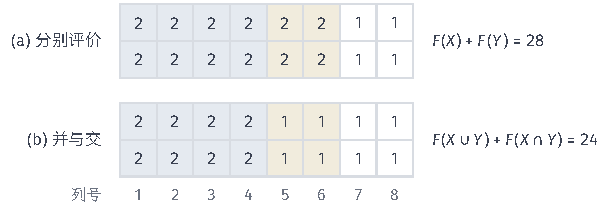
\includegraphics[width=103.258mm]{figures/01-basic-mathematics/04-graphs/tikz/c4-submodular-overlap-count/figure.pdf}
  \caption{覆盖函数上四值不等式的逐格计数，取$X=\{a,b\}$、$Y=\{b,c\}$。(a) 每格的数字是$X$与$Y$中覆盖它的组数，合计$F(X)+F(Y)$；(b) 每格的数字是$X\cup Y$与$X\cap Y=\{b\}$中覆盖它的组数，合计$F(X\cup Y)+F(X\cap Y)$。蓝底的第$1$至$4$列由公共部分覆盖，两边相同；黄底的第$5$、$6$列被$X$的$a$与$Y$的$c$分别覆盖而不被$b$覆盖，左边多计一次，四格合计正是差值$4$。}
  \label{fig:graph-setfn-submodular-overlap-count}
\end{figure}

\paragraph{割权的次模性}
割权按边累加，所以先看一条权为$w$的边$\{i,j\}$单独贡献的函数：它在$S$恰含$i,j$之一时取$w$，否则取$0$。对不是端点的元素，这条边的贡献不随它的加入而改变，增益为$0$。加入端点$i$时，若$j$已在集合中，这条边从跨越两侧变为两端同侧，增益为$-w$；若$j$不在集合中，这条边从两端同侧变为跨越两侧，增益为$+w$。

现在取$A\subseteq B$、$i\notin B$，按$j$的归属分三种情形比较两个增益，见图~\ref{fig:graph-setfn-cut-submodular-cases}。若$j\in A$，则$j$也在$B$中，两个增益都是$-w$；若$j\in B\setminus A$，则$\Delta(i\mid A)=+w$而$\Delta(i\mid B)=-w$；若$j\notin B$，两个增益都是$+w$。三种情形都满足$\Delta(i\mid A)\geq\Delta(i\mid B)$；待加入的元素不是这条边的端点时，两个增益都是$0$，不等式也成立。所以单条边的贡献是次模的。

由次模函数之和仍是次模函数，$\operatorname{cut}$作为各边贡献之和也是次模的。边权非负在这里是必要的：若某条边的权为负，第二种情形的不等号就反向了。

\begin{figure}[!htb]
  \centering
  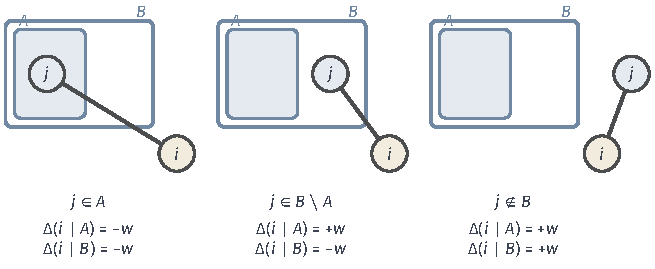
\includegraphics[width=110.723mm]{figures/01-basic-mathematics/04-graphs/tikz/c4-cut-submodular-cases/figure.pdf}
  \caption{割权函数次模性的逐边验证。固定一条权为$w\geq0$的边$\{i,j\}$，已选集合$A\subseteq B$（内框为$A$，外框为$B$），待加入的端点$i$（黄色）不在$B$中。按另一端点$j$的位置分三种情形：$j\in A$时两个增益都是$-w$；$j\in B\setminus A$时$A$上增益为$+w$、$B$上增益为$-w$；$j\notin B$时两个增益都是$+w$。每种情形都有$\Delta(i\mid A)\geq\Delta(i\mid B)$。}
  \label{fig:graph-setfn-cut-submodular-cases}
\end{figure}

\subsection{性质之间的关系}
\label{sec:graph-setfn-property-relations}

次模与单调互不蕴含。割权常常随集合增大而下降：$\operatorname{cut}(\varnothing)=\operatorname{cut}(V)=0$，而中间的子集可以有正的割权。图~\ref{fig:graph-setfn-property-counterexamples}(b)是只有一条权$1$的边的情形，割权依次为$0,1,1,0$，从单元素集到$\{1,2\}$时下降，所以次模函数不必单调。

反方向，图~\ref{fig:graph-setfn-property-counterexamples}(a)的函数
\[
  F(S)=\max\bigl\{3\,\mathbb I\{\{1,2\}\subseteq S\},\ \mathbb I\{3\in S\}\bigr\}
\]
是单调的，但$\Delta(2\mid\varnothing)=0<3=\Delta(2\mid\{1\})$，违反式~\eqref{eq:graph-setfn-diminishing-returns}，所以单调函数也不必次模。

\begin{figure}[!htb]
  \centering
  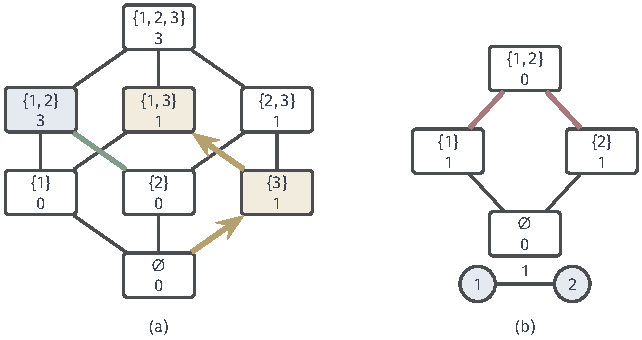
\includegraphics[width=108.687mm]{figures/01-basic-mathematics/04-graphs/tikz/c4-property-counterexamples/figure.pdf}
  \caption{单调性与次模性互不蕴含。每个框上行是子集，下行是函数值，连线连接只差一个元素的子集。(a) $F(S)=\max\{3\,\mathbb I\{\{1,2\}\subseteq S\},\mathbb I\{3\in S\}\}$：沿任一连线向上函数值不减，但绿色连线$\{2\}\to\{1,2\}$的增益$3$大于从空集加入$2$的增益$0$；黄色箭头是第~\ref{sec:graph-cardinality-selection}节贪心选择的路径，蓝色框是两元素时的最优集合。(b) 单条权$1$的边上的割权：次模，但红色连线上函数值从$1$降到$0$。}
  \label{fig:graph-setfn-property-counterexamples}
\end{figure}

\paragraph{超模函数}
把式~\eqref{eq:graph-setfn-diminishing-returns}的不等号反过来，即要求$\Delta(v\mid A)\leq\Delta(v\mid B)$，得到的函数称为\term{超模}函数（supermodular function）；等价地，$F$超模当且仅当$-F$次模。

超模描述的是协同：两个部件只有同时具备才能工作时，单独加入任何一个的增益都是$0$，在另一个已经存在时加入，增益才是正的。例如$F(S)=\mathbb I\{\{1,2\}\subseteq S\}$是超模的。

图~\ref{fig:graph-setfn-property-counterexamples}(a)的函数既不是次模也不是超模：元素$1,2$之间是协同的，而元素$3$与$\{1,2\}$之间是替代的，$\Delta(3\mid\varnothing)=1>0=\Delta(3\mid\{1,2\})$。模函数的增益恒为$w_v$，与已选集合无关，同时满足两个方向的不等式，所以它既是次模的也是超模的。

但同时次模和超模并不带来单调：由第~\ref{sec:graph-setfn-modularity}小节，模函数是否单调只取决于权重的符号。例如二元底集上取$c_0=0$、$w_1=1$、$w_2=-1$，则$F(\{1,2\})=0<1=F(\{1\})$，这个模函数既次模又超模，却不单调。

\paragraph{性质对照}
表~\ref{tab:graph-setfn-property-summary}汇总本节的函数（割权取图~\ref{fig:graph-setfn-property-counterexamples}(b)的单边图）。

表中尚未直接核对的几项如下：
\begin{itemize}
  \item 覆盖量：$\Delta(c\mid\varnothing)=8>4=\Delta(c\mid\{a\})$，增益随已选集合变小，所以不是超模的。
  \item 单边割权：$\Delta(1\mid\varnothing)=1>-1=\Delta(1\mid\{2\})$，所以不是超模的；$\operatorname{cut}(\{1\})+\operatorname{cut}(\{2\})=2\neq0=\operatorname{cut}(\{1,2\})+\operatorname{cut}(\varnothing)$，所以不是模函数。
  \item 净收益：它是次模函数$F$加上模函数$-c$，仍为次模。若它是模函数或超模函数，再加回模函数$c$，$F$也会是模函数或超模函数，与前两行矛盾；所以它同$F$一样既不是模函数也不是超模的。
  \item $\mathbb I\{\{1,2\}\subseteq S\}$：加入一个元素的增益只在另一元素已选时为$1$，随已选集合只增不减，所以是超模的；$\Delta(2\mid\varnothing)=0<1=\Delta(2\mid\{1\})$说明它不是次模的。
\end{itemize}

四种性质可以各种方式组合出现。所以后两章的算法保证都同时写明目标方向、函数是否单调、是否次模以及约束；只凭“次模”二字，不能决定采用哪种方法。

\begin{table}[!htb]
  \centering
  \caption{本节各函数的性质。“是”“否”均已在正文中由定义、判别式或反例核对；模函数同时满足次模与超模的不等式。}
  \label{tab:graph-setfn-property-summary}
  \small
  \begin{tabular}{@{}lcccc@{}}
    \toprule
    函数 & 单调 & 模 & 次模 & 超模 \\
    \midrule
    总成本$c$ & 是 & 是 & 是 & 是 \\
    覆盖量$F$ & 是 & 否 & 是 & 否 \\
    割权$\operatorname{cut}$ & 否 & 否 & 是 & 否 \\
    净收益$F-c$ & 否 & 否 & 是 & 否 \\
    $\mathbb I\{\{1,2\}\subseteq S\}$ & 是 & 否 & 否 & 是 \\
    图~\ref{fig:graph-setfn-property-counterexamples}(a)的函数 & 是 & 否 & 否 & 否 \\
    \bottomrule
  \end{tabular}
\end{table}

% 第8章第3节：子集累计与 Möbius 反演（子集格与累计；Möbius 反演及四元素算例；反演的计算：逐元素差分；有限偏序集上的推广）。

\section{子集累计与 Möbius 反演}
\label{sec:comb-cumulative-inversion}

设想每个课程组合有一个总得分：单门课各有自己的贡献，某两门课同时选又会产生额外的配合效果，配合也可能是负的。能观察到的是每个组合的总得分，想知道的却是每个组合\emph{自身}贡献了多少。

卷一计数中的容斥原理由各交集的大小恢复并集的大小，这里做的是同一类“由累计量恢复局部量”的事，只是对象换成了一般的数值。本节只用有限求和与包含关系，不依赖上一节的单调或次模假设，也不是后面选择算法的前提。

\subsection{子集格与累计}
\label{sec:graph-setfn-subset-lattice}

累计沿包含关系进行，所以先把包含关系画出来。包含关系是幂集上的偏序：每个集合包含自身；$S\subseteq T$与$T\subseteq S$同时成立时$S=T$；包含关系可以传递。有限集合$V$的全部子集连同包含关系称为$V$的\term{子集格}（subset lattice）：两个子集的交是它们最大的公共子集，并是包含两者的最小集合。

图~\ref{fig:comb-mobius-cumulative-local}按元素个数自下而上分层画出$V_0=\{1,2,3,4\}$的子集格，每条连线连接只差一个元素的两个子集，沿连线向上一步就是加入一个元素。图~\ref{fig:graph-setfn-subset-binary-cube}中的立方体正是三元底集的子集格。

从$S$出发沿连线一路向下能到达的子集，恰好是$S$的全部子集，例如从$\{1,3\}$向下只能到达$\{1\}$、$\{3\}$和空集。累计值就沿这些向下的路径收集贡献。

\begin{figure}[!htb]
  \centering
  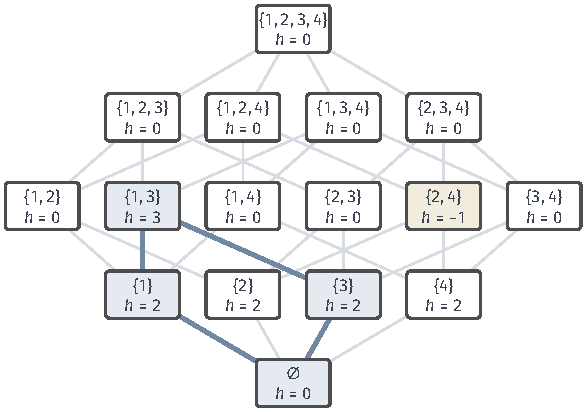
\includegraphics[width=99.187mm]{figures/01-basic-mathematics/04-graphs/tikz/c4-subset-lattice-cumulative/figure.pdf}
  \caption{四元素集合$V_0=\{1,2,3,4\}$的子集格与各子集自身的贡献$h$。子集按元素个数自下而上分层，连线连接只差一个元素的两个子集；框内上行为子集，下行为教学设定的贡献。蓝色标出$\{1,3\}$及其全部子集，它们的贡献相加得到累计值$g(\{1,3\})=0+2+2+3=7$；黄色框$\{2,4\}$的自身贡献为负。}
  \label{fig:comb-mobius-cumulative-local}
\end{figure}

\paragraph{自身贡献与累计值}
给每个子集$T$指定一个实数$h(T)$，表示$T$作为整体\emph{自身}带来的贡献：单元素集的贡献是单门课的得分，二元集的贡献是两门课在各自得分之外的配合效果，依此类推。$S$的累计值收集它的全部子集的贡献：
\begin{equation}
  g(S)=\sum_{T\subseteq S}h(T).
  \label{eq:comb-zeta-transform}
\end{equation}
$g$与$h$都是$V$上的集合函数。累计不只相加单元素的贡献，$S$内部更大子集的配合贡献也计入其中。

图~\ref{fig:comb-mobius-cumulative-local}的教学设定让四个单项各贡献$2$，$\{1,3\}$另有配合贡献$3$，$\{2,4\}$另有配合贡献$-1$，其余子集（包括空集和全部三元、四元子集）的贡献为$0$。于是
\[
  g(\{1,3\})=h(\varnothing)+h(\{1\})+h(\{3\})+h(\{1,3\})=0+2+2+3=7,
\]
而两个单项的累计值之和只有$g(\{1\})+g(\{3\})=4$，多出的$3$正是$\{1,3\}$自身的贡献。

反演处理相反方向的问题：已知全部$2^n$个累计值$g(S)$，求全部$2^n$个自身贡献$h(S)$，使它们按式~\eqref{eq:comb-zeta-transform}累计后恰好给出已知的$g$。需要回答的是这样的$h$是否存在、是否唯一，以及怎样算出来。

\subsection{Möbius 反演}
\label{sec:graph-setfn-mobius-inversion}

先看一列数的情形。若$g_k=h_1+\cdots+h_k$是前缀和，恢复$h_k$只需相邻两项相减：
\[
  h_k=g_k-g_{k-1}.
\]
子集格上的累计也是一种“前缀和”，只是$S$的下方不止一个紧邻的子集，而有$|S|$个$S\setminus\{i\}$，每个元素给出一个相减的方向。只沿一个方向相减还不够，各个方向的差会把某些贡献重复减去，需要再加回来。

两元素的情形可以完整写出。$g(\{1,3\})$包含$h(\varnothing)$、$h(\{1\})$、$h(\{3\})$和$h(\{1,3\})$四项。为了只留下$h(\{1,3\})$，先减去
\[
  g(\{1\})=h(\varnothing)+h(\{1\}),\qquad g(\{3\})=h(\varnothing)+h(\{3\}),
\]
两个单项贡献被去掉，但$h(\varnothing)$被多减了一次，再加回$g(\varnothing)=h(\varnothing)$，剩下的恰是
\[
  h(\{1,3\})=g(\{1,3\})-g(\{1\})-g(\{3\})+g(\varnothing).
\]

表~\ref{tab:graph-setfn-mobius-cancellation}逐项记录四个累计值各含哪些贡献、带什么符号：按列相加，$h(\varnothing)$、$h(\{1\})$、$h(\{3\})$的系数都抵消为$0$，只有$h(\{1,3\})$留下系数$1$。

同一个式子也是两次相邻差：
\[
  h(\{1,3\})=\bigl(g(\{1,3\})-g(\{3\})\bigr)-\bigl(g(\{1\})-g(\varnothing)\bigr),
\]
两个括号各沿“加入元素$1$”的方向相减，括号之间再沿“加入元素$3$”的方向相减。展开后，每个$g(T)$的符号由$T$比$S$少几个元素决定，少一个变一次号。一般情形的公式正是这样，称为\term{Möbius反演}（Möbius inversion）。

\begin{table}[!htb]
  \centering
  \begin{tabular}{@{}lcccc@{}}
    \toprule
    & $h(\varnothing)$ & $h(\{1\})$ & $h(\{3\})$ & $h(\{1,3\})$ \\
    \midrule
    $+g(\{1,3\})$ & $+1$ & $+1$ & $+1$ & $+1$ \\
    $-g(\{1\})$ & $-1$ & $-1$ & & \\
    $-g(\{3\})$ & $-1$ & & $-1$ & \\
    $+g(\varnothing)$ & $+1$ & & & \\
    \midrule
    合计 & $0$ & $0$ & $0$ & $1$ \\
    \bottomrule
  \end{tabular}
  \caption{$h(\{1,3\})=g(\{1,3\})-g(\{1\})-g(\{3\})+g(\varnothing)$中各项的抵消。每行把一个累计值按式~\eqref{eq:comb-zeta-transform}展开，记下各贡献的系数（已乘上该累计值前的符号），空白为$0$；末行按列相加。}
  \label{tab:graph-setfn-mobius-cancellation}
\end{table}

\begin{theorem}[子集格上的 Möbius 反演]
\label{thm:comb-mobius-inversion}
设$V$为有限集合，$g,h:\mathcal P(V)\to\mathbb R$。若对每个$S\subseteq V$式~\eqref{eq:comb-zeta-transform}成立，则对每个$S\subseteq V$有
\begin{equation}
  h(S)=\sum_{T\subseteq S}(-1)^{|S|-|T|}g(T).
  \label{eq:comb-mobius-inversion}
\end{equation}
反过来，若对每个$S$式~\eqref{eq:comb-mobius-inversion}成立，则式~\eqref{eq:comb-zeta-transform}也对每个$S$成立。
\end{theorem}

\begin{proof}
把式~\eqref{eq:comb-zeta-transform}代入式~\eqref{eq:comb-mobius-inversion}右侧，得到对全部满足$R\subseteq T\subseteq S$的集合对$(R,T)$的双重和。先固定$T$再取$R$，与先固定$R$再取$T$，遍历的是同一批有限个集合对；有限和只是把这些项全部相加，与分组次序无关，所以可以交换求和次序：
\[
  \begin{aligned}
  &\sum_{T\subseteq S}(-1)^{|S|-|T|}\sum_{R\subseteq T}h(R)\\
  &\qquad=\sum_{R\subseteq S}h(R)\sum_{T:\,R\subseteq T\subseteq S}(-1)^{|S|-|T|}.
  \end{aligned}
\]
固定$R$后，满足$R\subseteq T\subseteq S$的$T$由$S\setminus R$中哪些元素被加入决定，即$T=R\cup D$，$D\subseteq S\setminus R$任意，且$|S|-|T|=|S\setminus R|-|D|$。记$q=|S\setminus R|$，按$|D|=j$分组，大小为$j$的$D$有$\binom qj$个，所以内层和等于
\[
  \begin{aligned}
  \sum_{j=0}^{q}\binom qj(-1)^{q-j}&=(-1)^q\sum_{j=0}^{q}(-1)^j\binom qj\\
  &=\begin{cases}1,&q=0,\\0,&q\geq1,\end{cases}
  \end{aligned}
\]
最后一步用组合数的交错和：$q\geq1$时，$q$元集合中偶数大小的子集与奇数大小的子集一样多（固定一个元素，加入或删去它就把两类一一配对），所以$\sum_{j=0}^{q}(-1)^j\binom qj=0$。

内层和只在$R=S$时为$1$，在$R$是$S$的真子集时为$0$，所以真子集上的贡献全部抵消，右侧只剩$h(S)$。表~\ref{tab:graph-setfn-mobius-cancellation}的各列合计正是$S=\{1,3\}$时的这些内层和。

反方向同样直接核对。由式~\eqref{eq:comb-mobius-inversion}给出$h$，代入$\sum_{T\subseteq S}h(T)$并交换求和次序，
\[
  \sum_{T\subseteq S}h(T)=\sum_{R\subseteq S}g(R)\sum_{T:\,R\subseteq T\subseteq S}(-1)^{|T|-|R|}.
\]
仍写$T=R\cup D$，内层和等于$\sum_{j=0}^{q}(-1)^j\binom qj$，它在$R=S$时只有$D=\varnothing$一项而等于$1$，在$R\neq S$时为$0$。所以右侧等于$g(S)$。
\end{proof}

定理回答了存在与唯一的问题。对任意给定的$g$，按式~\eqref{eq:comb-mobius-inversion}定义的$h$累计后恰好回到$g$，所以所求的$h$存在；而任何满足式~\eqref{eq:comb-zeta-transform}的$h$都必须等于式~\eqref{eq:comb-mobius-inversion}的右侧，所以它是唯一的。

式~\eqref{eq:comb-zeta-transform}与式~\eqref{eq:comb-mobius-inversion}是一对互逆的变换：从贡献到累计，再从累计回到贡献，不丢失任何信息。

证明中起作用的是组合数的交错和为零，这与容斥原理相同；区别在于容斥使并集中每个元素恰计一次，反演只保留指定子集自身的贡献。

\paragraph{四元素算例}
仍用指示函数$\mathbb I\{\cdot\}$，沿用图~\ref{fig:comb-mobius-cumulative-local}的设定，累计值可以写成
\[
  g(S)=2|S|+3\,\mathbb I\{\{1,3\}\subseteq S\}-\mathbb I\{\{2,4\}\subseteq S\}.
\]
其中$2|S|$收集$S$中各单项的贡献，后两项在$S$包含$\{1,3\}$或$\{2,4\}$时计入相应的配合贡献。表~\ref{tab:comb-four-element-mobius}列出全部$16$个累计值，以及只用这些累计值按式~\eqref{eq:comb-mobius-inversion}恢复的贡献。

\begin{table}[!htb]
  \centering
  \begin{tabular}{ccc@{\qquad}ccc}
    \toprule
    $S$ & $g(S)$ & $h(S)$ & $S$ & $g(S)$ & $h(S)$ \\
    \midrule
    $\varnothing$ & $0$ & $0$ & $\{2,3\}$ & $4$ & $0$ \\
    $\{1\}$ & $2$ & $2$ & $\{2,4\}$ & $3$ & $-1$ \\
    $\{2\}$ & $2$ & $2$ & $\{3,4\}$ & $4$ & $0$ \\
    $\{3\}$ & $2$ & $2$ & $\{1,2,3\}$ & $9$ & $0$ \\
    $\{4\}$ & $2$ & $2$ & $\{1,2,4\}$ & $5$ & $0$ \\
    $\{1,2\}$ & $4$ & $0$ & $\{1,3,4\}$ & $9$ & $0$ \\
    $\{1,3\}$ & $7$ & $3$ & $\{2,3,4\}$ & $5$ & $0$ \\
    $\{1,4\}$ & $4$ & $0$ & $V_0$ & $10$ & $0$ \\
    \bottomrule
  \end{tabular}
  \caption{四元素子集格上的累计值$g$与由式~\eqref{eq:comb-mobius-inversion}恢复的自身贡献$h$。恢复结果与教学设定一致：四个单项各为$2$，$\{1,3\}$为$3$，$\{2,4\}$为$-1$，其余子集（包括全部三元子集和$V_0$）均为$0$。}
  \label{tab:comb-four-element-mobius}
\end{table}

逐个套用公式，两个二元子集的贡献按前面的四项公式恢复：
\[
  h(\{1,3\})=7-2-2+0=3,\qquad h(\{2,4\})=3-2-2+0=-1.
\]

三元子集要用到八个累计值。对$S=\{1,2,3\}$，按子集大小依次取三元、二元、一元和空集项，
\[
  h(\{1,2,3\})=9-(4+7+4)+(2+2+2)-0=0.
\]
虽然$\{1,2,3\}$包含有配合效果的$\{1,3\}$，它的累计值$9$也大于三个单项之和$6$，但多出的$3$已经由$h(\{1,3\})$解释，三门课之间没有新的整体效果，所以三元贡献为$0$。

$\{1,3,4\}$也是如此：$g=9$，恢复出$h=0$。其余两个三元子集同样得到$0$，例如
\[
  h(\{2,3,4\})=5-(4+3+4)+(2+2+2)-0=0,
\]
其中$-1$的配合贡献已由$h(\{2,4\})$解释。反演还允许贡献为负，$h(\{2,4\})=-1$就是一例。

\subsection{反演的计算}
\label{sec:graph-setfn-mobius-computation}

\subsubsection{问题与思路}

输入是全部$2^n$个累计值，输出是全部$2^n$个自身贡献。直接套用式~\eqref{eq:comb-mobius-inversion}，计算$h(S)$要读取$S$的全部$2^{|S|}$个子集上的累计值。

另一种做法是由式~\eqref{eq:comb-zeta-transform}移项逐个求解：
\[
  h(S)=g(S)-\sum_{T\subsetneq S}h(T).
\]
从$h(\varnothing)=g(\varnothing)$出发，按元素个数从小到大计算，算到$S$时它的全部真子集的$h$都已求出。在四元素算例中，先得到$h(\varnothing)=0$和单项贡献$2$，再得二元贡献，例如
\[
  h(\{1,3\})=7-(0+2+2)=3,
\]
最后得到三元贡献，例如
\[
  h(\{1,2,3\})=9-(0+2+2+2+0+3+0)=0.
\]

这种递推同样要对每个$S$遍历它的全部子集。$k$元子集有$\binom nk$个，各有$2^k$个子集，所以由二项式定理，两种做法读取的项数都是
\[
  \sum_{k=0}^{n}\binom nk2^k=3^n.
\]
两种做法的共同瓶颈是每个$S$都要单独遍历它的全部子集。

上一小节把单个值$h(\{1,3\})$写成了两次相邻差，这提示可以按元素而不是按子集组织计算。式~\eqref{eq:comb-mobius-inversion}中的符号可以按元素拆开：对$T\subseteq S$，$(-1)^{|S|-|T|}$是$S\setminus T$中每个元素各贡献一个$-1$的乘积。于是交错和可以一个元素一个元素地做：先对全部子集沿“加入元素$1$”的方向取相邻差，再在结果上沿元素$2$的方向取差，依此类推。

每个元素只处理一轮，一轮对$2^{n-1}$对相邻子集各做一次减法，不再为每个$S$单独遍历它的子集。这种做法称为逐元素差分。

\subsubsection{算法实现}

元素的编号$1,\ldots,n$与子集在数组中的位置在开始前确定，运行中不再改变，所以不把它们计入算法的状态。

\paragraph{子集数组的数据结构}
数组以子集为下标。沿用第~\ref{sec:graph-setfn-binary-vectors}小节的指示向量，把$S$的指示向量$(x_1,\ldots,x_n)$读成二进制数$\sum_{i=1}^{n}x_i2^{i-1}$，作为$S$在长度为$2^n$的数组中的位置。$S$含元素$i$，当且仅当这个数从低位数起的第$i$位为$1$；这时$S\setminus\{i\}$的位置是它减去$2^{i-1}$。例如$n=3$时$\{1,3\}$的位置是$101_2=5$，$\{1,3\}\setminus\{1\}=\{3\}$的位置是$5-1=4$。

依次扫描位置$0,1,\ldots,2^n-1$，挑出第$i$位为$1$的位置，就把含$i$的子集各访问一次，每次用一次减法找到$S\setminus\{i\}$。

\paragraph{逐元素差分的实现}
算法维护两项状态：
\begin{itemize}
  \item 数组$a(\cdot)$：以子集为下标，长度为$2^n$，初值$a(S)=g(S)$；
  \item 当前元素$i$：本轮处理的元素，初值为$1$。
\end{itemize}
第$i$轮按子集是否含$i$分别处理，处理完令$i\gets i+1$：
\begin{itemize}
  \item 含$i$的子集$S$：令$a(S)\gets a(S)-a(S\setminus\{i\})$；
  \item 不含$i$的子集：保持不变。
\end{itemize}
本轮读取的$a(S\setminus\{i\})$所在的子集不含$i$，本轮不会被修改，所以更新可以原地进行，不需要另存上一轮的数组。处理完元素$n$后停止，输出$a$。在子集格上看，第$i$轮只沿“加入元素$i$”方向的连线做差，图~\ref{fig:graph-setfn-subset-binary-cube}中同色的一组边就是一轮读取的方向。

\begin{algorithm}[逐元素差分]
\label{alg:graph-setfn-mobius-coordinate}
输入：底集$V=\{1,\ldots,n\}$上的全部累计值$g(S)$。输出：全部自身贡献$h(S)$。
\begin{enumerate}
  \item 对每个$S\subseteq V$置$a(S)=g(S)$；令$i=1$。
  \item 对每个含$i$的子集$S$，置$a(S)=a(S)-a(S\setminus\{i\})$；不含$i$的子集不变。
  \item 若$i<n$，令$i\gets i+1$并回到第2步；否则输出$h(S)=a(S)$。
\end{enumerate}
\end{algorithm}

\paragraph{执行过程}
先在三元子集格$\{1,2,3\}$上执行。四元素设定限制到$\{1,2,3\}$的子集上，仍是同一组累计值与贡献，因为$g(S)$和$h(S)$只读取$S$的子集。

初始数组就是累计值：
\[
  \begin{gathered}
  a(\varnothing)=0,\qquad a(\{1\})=a(\{2\})=a(\{3\})=2,\\
  a(\{1,2\})=4,\quad a(\{1,3\})=7,\quad a(\{2,3\})=4,\quad a(\{1,2,3\})=9.
  \end{gathered}
\]

\begin{BookInlineFigure}
  \centering
  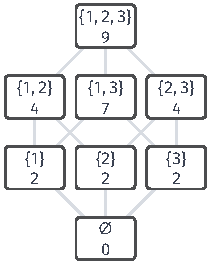
\includegraphics[width=35.736mm]{figures/03-graphs/03-set-functions-and-subset-selection/tikz/reading-steps/mobius-round-0.pdf}
  \caption{逐元素差分的初始状态：每个框的上行是子集$S$，下行是累计值$g(S)$。本例取四元素设定限制到$\{1,2,3\}$的值。}
  \label{fig:graph-setfn-mobius-coordinate-rounds}
\end{BookInlineFigure}

每轮只改动含被处理元素的四个子集：
处理元素$1$：$\{1\}$为$2-0=2$，$\{1,2\}$为$4-2=2$，$\{1,3\}$为$7-2=5$，$\{1,2,3\}$为$9-4=5$。
\begin{BookInlineFigure}
  \centering
  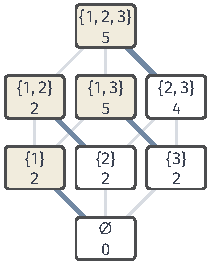
\includegraphics[width=35.736mm]{figures/03-graphs/03-set-functions-and-subset-selection/tikz/reading-steps/mobius-round-1.pdf}
  \caption{处理元素$1$后的数组。黄色子集含$1$；蓝色粗线连接该子集与本轮读取的$S\setminus\{1\}$，框内下行已写入相减后的值。}
  \label{fig:graph-setfn-mobius-coordinate-rounds-1}
\end{BookInlineFigure}

处理元素$2$：$\{2\}$为$2-0=2$，$\{1,2\}$为$2-2=0$，$\{2,3\}$为$4-2=2$，$\{1,2,3\}$为$5-5=0$。
\begin{BookInlineFigure}
  \centering
  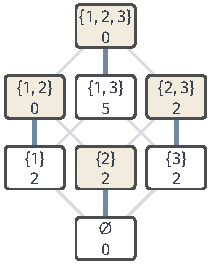
\includegraphics[width=35.736mm]{figures/03-graphs/03-set-functions-and-subset-selection/tikz/reading-steps/mobius-round-2.pdf}
  \caption{处理元素$2$后的数组。本轮只沿蓝色粗线做差，改写含$2$的四个黄色子集；其余值保持不变。}
  \label{fig:graph-setfn-mobius-coordinate-rounds-2}
\end{BookInlineFigure}

处理元素$3$：$\{3\}$为$2-0=2$，$\{1,3\}$为$5-2=3$，$\{2,3\}$为$2-2=0$，$\{1,2,3\}$为$0-0=0$。
\begin{BookInlineFigure}
  \centering
  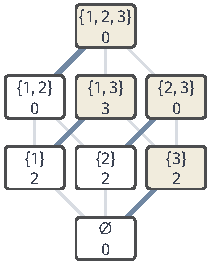
\includegraphics[width=35.736mm]{figures/03-graphs/03-set-functions-and-subset-selection/tikz/reading-steps/mobius-round-3.pdf}
  \caption{处理元素$3$后的数组，即自身贡献$h$。此时$h(\{1,3\})=3$，单项贡献各为$2$，其余值为$0$。}
  \label{fig:graph-setfn-mobius-coordinate-rounds-3}
\end{BookInlineFigure}

最终数组就是$h$：单项各为$2$，$h(\{1,3\})=3$，其余为$0$。

$\{1,3\}$的值$7\to5\to5\to3$正是上一小节的两次相邻差：处理元素$1$时减去$g(\{3\})$，处理元素$3$时减去已经差分过的$a(\{1\})=g(\{1\})-g(\varnothing)$。图~\ref{fig:graph-setfn-mobius-coordinate-rounds-1}至图~\ref{fig:graph-setfn-mobius-coordinate-rounds-3}分别给出各轮结束后的状态。


四元素算例照样做四轮，每轮改动含$i$的$8$个子集，最后的数组与表~\ref{tab:comb-four-element-mobius}中的$h$逐项一致。例如$\{2,4\}$依次为$3,3,1,1,-1$：处理元素$2$时减去$a(\{4\})=2$，处理元素$4$时减去当前的$a(\{2\})=2$。中间各轮的数组只是部分差分，只有最后一轮之后才是$h$。

\subsubsection{算法分析}

\paragraph{正确性}
上面按元素拆分符号的说法，可以由一个不变式精确表达。记$[i]=\{1,\ldots,i\}$。断言：处理完元素$1,\ldots,i$后，
\[
  a(S)=\sum_{\substack{T\subseteq S\\ T\setminus[i]=S\setminus[i]}}(-1)^{|S|-|T|}g(T),
\]
即只对那些与$S$在元素$i+1,\ldots,n$上一致的子集$T$做交错求和。$i=0$时条件迫使$T=S$，右侧就是$g(S)$，与初始化一致。

设断言对$i$成立，看第$i+1$轮。若$i+1\notin S$，$a(S)$不变；而$S$的子集都不含$i+1$，“在$i+1,\ldots,n$上一致”与“在$i+2,\ldots,n$上一致”是同一个条件，断言对$i+1$成立。

若$i+1\in S$，新值是
\[
  a(S)-a(S\setminus\{i+1\}).
\]
前一项求和的$T$与$S$在$i+1,\ldots,n$上一致，因而含$i+1$；后一项求和的$T$与$S\setminus\{i+1\}$一致，因而不含$i+1$，符号$(-1)^{|S|-1-|T|}$再乘以$-1$变成$(-1)^{|S|-|T|}$。两组$T$合起来，恰是与$S$在$i+2,\ldots,n$上一致的全部子集，断言对$i+1$成立。

取$i=n$，条件不再限制$T$，右侧正是式~\eqref{eq:comb-mobius-inversion}，所以输出就是$h$。

\paragraph{复杂度}
逐元素差分每轮做$2^{n-1}$次减法，共$n2^{n-1}$次；按上面的数据结构，每次找到$S\setminus\{i\}$只需一次整数减法，原地更新只用长度为$2^n$的数组。逐个套用公式与按子集大小递推都需要$3^n$次运算，四元素算例中是$32$次对$81$次。

不过输入本身已有$2^n$个数，三种方式的运算量都随$n$指数增长。逐元素差分降低的是指数的底，从$3$降到$2$，并没有使计算摆脱指数规模。

\paragraph{累计方向}
把每一轮的减号换成加号、从$a=h$出发做$n$轮，同样的归纳（不变式中的符号$(-1)^{|S|-|T|}$换成$1$，$g$换成$h$）说明得到的是累计值$g$。例如$\{1,3\}$由$3$经$3+2=5$、$5+2=7$回到$g(\{1,3\})$。所以累计和反演可以用同一套逐元素扫描完成，开销也相同。

\subsection{有限偏序集上的推广}
\label{sec:graph-setfn-poset-mobius}

反演公式中的系数$(-1)^{|S|-|T|}$只依赖两个子集的相对位置。同样的问题可以在任意有限偏序集$(X,\preceq)$上提出：给每个元素$y$一个数$h(y)$，沿下方累计得
\[
  g(x)=\sum_{y\preceq x}h(y),
\]
再问怎样由$g$恢复$h$。这时系数不再一律是$\pm1$，而由下面的函数确定。

\begin{definition}[Möbius 函数]
\label{def:graph-setfn-mobius-function}
设$(X,\preceq)$是有限偏序集，记$y\prec x$表示$y\preceq x$且$y\neq x$。偏序集的\term{Möbius函数}（Möbius function）$\mu$对满足$y\preceq x$的元素对定义为
\begin{equation}
  \mu(y,y)=1,\qquad \mu(y,x)=-\sum_{z:\,y\preceq z\prec x}\mu(y,z)\quad(y\prec x),
  \label{eq:graph-setfn-mobius-function-def}
\end{equation}
对不满足$y\preceq x$的元素对取$\mu(y,x)=0$。
\end{definition}

定义固定区间的下端$y$，从对角值$\mu(y,y)=1$出发向上递推：算$\mu(y,x)$时只用到区间$\{z:y\preceq z\prec x\}$上已经算出的值，而有限偏序集保证递推在有限步内完成。递推式移项后写成
\begin{equation}
  \sum_{z:\,y\preceq z\preceq x}\mu(y,z)=0\qquad(y\prec x),
  \label{eq:graph-setfn-mobius-function-sum}
\end{equation}
即每个非平凡区间上的系数之和为零；$y=x$时这个和是$\mu(y,y)=1$。

这一抵消性质足以完成反演，论证分两步。先定义
\[
  \tilde h(x)=\sum_{y\preceq x}\mu(y,x)g(y),
\]
并验证它累计后回到$g$。对任意$s\in X$，交换有限和的次序，
\[
  \begin{aligned}
  \sum_{x\preceq s}\tilde h(x)&=\sum_{x\preceq s}\sum_{y\preceq x}\mu(y,x)g(y)\\
  &=\sum_{y\preceq s}g(y)\sum_{x:\,y\preceq x\preceq s}\mu(y,x).
  \end{aligned}
\]
由式~\eqref{eq:graph-setfn-mobius-function-sum}，内层和在$y\prec s$时为$0$，在$y=s$时为$1$，所以右侧等于$g(s)$。

再说明满足累计式的$h$只有一个。累计式可以写成
\[
  h(x)=g(x)-\sum_{y\prec x}h(y),
\]
右侧只用到严格位于$x$下方的元素。把有限偏序集的元素排成一列，使每个元素都排在它上方的元素之前（例如反复取出当前剩余元素中的一个极小元），按这个次序逐个计算，$h$的每个值都被$g$唯一确定。$\tilde h$也满足累计式，所以$h=\tilde h$，即
\begin{equation}
  h(x)=\sum_{y\preceq x}\mu(y,x)g(y).
  \label{eq:graph-setfn-poset-mobius-inversion}
\end{equation}

在子集格上，$\mu(T,S)=(-1)^{|S|-|T|}$满足这个递推：对$T\subsetneq S$，记$q=|S\setminus T|\geq1$，
\[
  \sum_{R:\,T\subseteq R\subseteq S}(-1)^{|R|-|T|}=\sum_{j=0}^{q}(-1)^j\binom qj=0.
\]
由于递推从$\mu(T,T)=1$出发唯一确定全部值，子集格上的Möbius函数就是$(-1)^{|S|-|T|}$，只取$\pm1$，式~\eqref{eq:comb-mobius-inversion}是一般反演式的特例。

\paragraph{整除偏序}
图~\ref{fig:graph-setfn-mobius-divisors}是$12$的六个正因数在整除关系下的偏序。从$\mu(1,1)=1$出发，先得$\mu(1,2)=\mu(1,3)=-1$。区间$\{1,2,4\}$是一条链，区间$\{1,2,3,6\}$与两元素的子集格形状相同，从$1$到$12$的区间含全部六个因数。按定义逐个递推，
\[
  \begin{aligned}
  \mu(1,4)&=-(1-1)=0,\\
  \mu(1,6)&=-(1-1-1)=1,\\
  \mu(1,12)&=-(1-1-1+0+1)=0.
  \end{aligned}
\]
系数出现了$0$，说明一般偏序上的反演确实不同于子集格上的交错加减。

这一推广只是补充，后两章的选择算法都不以它为前提。

\begin{figure}[!htb]
  \centering
  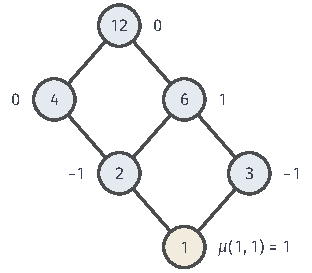
\includegraphics[width=52.613mm]{figures/01-basic-mathematics/04-graphs/tikz/c4-mobius-divisor-poset/figure.pdf}
  \caption{$12$的正因数在整除关系下的偏序，连线连接直接相邻的两个因数，下方整除上方。节点旁的数是$\mu(1,x)$，由$\mu(1,1)=1$（黄色节点）自下而上递推得到。链$1\mid2\mid4$上$\mu(1,4)=0$，与子集格同形的区间$\{1,2,3,6\}$上$\mu(1,6)=1$。}
  \label{fig:graph-setfn-mobius-divisors}
\end{figure}

\FloatBarrier
\section{本章小结}
\label{sec:set-functions-chapter-summary}

本章从传感器覆盖出发，把对整组选择的评价写成有限底集上的集合函数。底集可以是传感器，也可以是图的顶点或边，不必带图结构。$n$元底集的完整取值表有$2^n$项，所以函数通常由求值规则给出，算法的代价要分开计入求值次数和每次求值的开销。指示向量把子集换成零一向量，只换了索引方式，不带来可加性或局部分解。边际增益$\Delta(v\mid S)$是后面一切判别的基本量：它依赖已选集合，沿任一加入次序累加，总和等于两端函数值之差。

用边际增益可以分别回答三个问题。单调性问新增元素会不会降低评价，等价于全部边际增益非负；模性问每个元素的贡献是否固定，等价于四值等式，模函数恰是常数加固定权重之和；次模性问收益是否随已选集合增大而递减，在有限底集上与四值不等式等价。覆盖量与非负边权的割权是次模的典型例子，协同效应则给出超模函数。

这些性质互不蕴含。割权次模而不单调；$\max\{3\,\mathbb I\{\{1,2\}\subseteq S\},\mathbb I\{3\in S\}\}$中元素$1,2$只有同时选中才有大价值，它单调而不次模；模函数同时次模和超模，却可能因为负权重而不单调。归一化只是减去常数$F(\varnothing)$的约定，不改变任何边际增益。所以后面引用某种算法保证时，要逐项写明它需要哪些性质，不能只凭“次模”判断。

子集累计与Möbius反演回答另一个问题：由全部累计值恢复每个子集自身的贡献。反演按元素个数之差交替加减，依靠的是组合数交错和为零的抵消，它与累计互为逆变换，结果可以为负。这一问题只依赖有限求和与包含关系，不需要单调或次模。计算上，逐个套用公式和按子集大小递推都要$3^n$次运算，逐元素差分降到$n2^{n-1}$次，但仍随底集大小指数增长。一般有限偏序集上，Möbius函数由区间递推确定，子集格上的交替符号是它的特例。

下一章利用本章的边际增益和次模性，在基数或预算约束下最大化集合函数；第~\ref{chap:pairwise-binary-minimization}章再把一类可分解为一元项与成对项的次模函数化为割，精确求最小值。

